The question of choosing an interesting hash function family is very important in our problem because we often have to hash elements, in order to be able to store data or to test the membership of an element in a set. Therefore we want the hash functions to be fast to compute while being independant. In particular we will look for a set of hash functions that hashes integers in the set $\{0,\cdots,m-1\}$ :
\begin{enumerate}
 \item The multiplication method : we assume that we have a real number generator. We generate the hash family $h_{\theta} :  x \rightarrow \left \lfloor m \mathrm{frac}(x\times \theta) \right \rfloor$ where $0<\theta<1$ is a random real number.
 \item The less hashing method : we assume that we have two hash functions $h_a$ and $h_b$ hashing integers to the set $\{0,\cdots,m-1\}$, we can generate the hash function family $\mathcal{H} = \{
 x \rightarrow h_a(x) + i h_b(x) 
 \mathrm{\ mod\ } m
 , i \in 
 \{0,\cdots,k-1\} 
 \}$.
\end{enumerate}

\begin{figure}[H]
\centering
 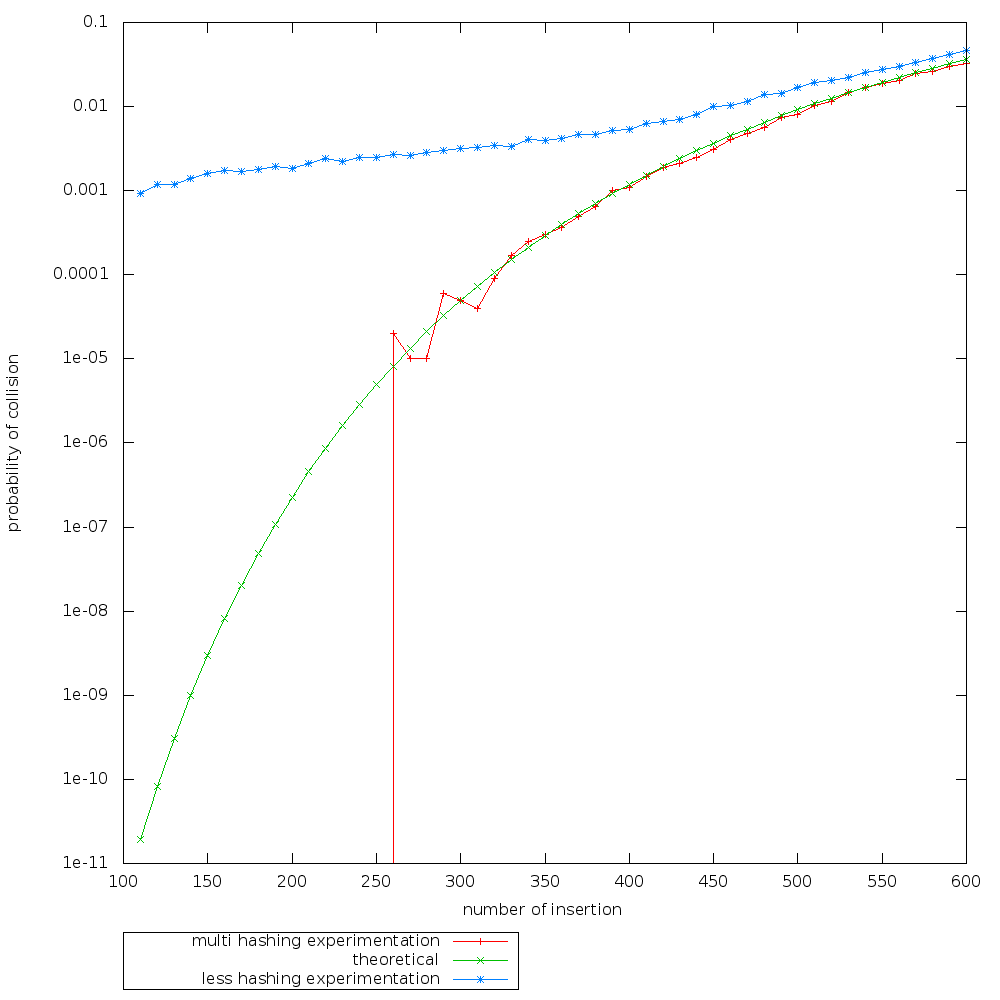
\includegraphics[width = 0.5\linewidth]{./image/bf/false_positive_probability.png}
 \caption{Testing the probability of getting a false positive with two different families of Hash functions} \label{fig:fpp}
\end{figure}
\paragraph{} The graphic above shows that the less hashing method, even if easy to compute, can not be used in our case because of the high probability of getting false positive. However this hashing method could be really interesting when hashing in a space of size $m$ growing linearly in the number of added element, because then it has the same asymptotic behaviour than an independant hash family (see \cite{DBLP:journals/rsa/KirschM08}). Such a growth of the size of the hashing space can not be used in our case where we assumed that we have no bound on the size of the history. Therefore we shall use the multiplication method which needs more computation but is more reliable, and the figure~\ref{fig:fpp} enables us to choose the number of elements we can insert in a slice given a bound on the probability of false positive.